\documentclass[11pt,a4paper,oneside]{report}             % Single-side
%\documentclass[11pt,a4paper,twoside,openright]{report}  % Duplex

%\PassOptionsToPackage{chapternumber=Huordinal}{magyar.ldf}
\usepackage{t1enc}
\usepackage[latin2]{inputenc}
\usepackage{amsmath}
\usepackage{amssymb}
\usepackage{enumerate}
\usepackage[thmmarks]{ntheorem}
\usepackage{graphics}
\usepackage{booktabs}
\usepackage{multirow}
\usepackage{xytree}
\usepackage{tikz-dependency}
\usepackage{float}
\usepackage{epsfig}
\usepackage{listings}
\usepackage{color}
%\usepackage{fancyhdr}
\usepackage{lastpage}
\usepackage{anysize}
\usepackage[english]{babel}
\usepackage{sectsty}
\usepackage{setspace}  % Ettol a tablazatok, abrak, labjegyzetek maradnak 1-es sorkozzel!
\usepackage[hang]{caption}
\usepackage{hyperref}
\usepackage{placeins}

%--------------------------------------------------------------------------------------
% Main variables
%--------------------------------------------------------------------------------------
\newcommand{\vikszerzo}{Kov\'acs \'Ad\'am}
\newcommand{\vikkonzulens}{Dr.~Recski G\'abor}
\newcommand{\vikcim}{Semantic parsing with graph transformations}
\newcommand{\viktanszek}{Department of Automation and Applied Informatics}
\newcommand{\vikdoktipus}{Master's Thesis}
\newcommand{\vikdepartmentr}{Kov\'acs \'Ad\'am}

%--------------------------------------------------------------------------------------
% Page layout setup
%--------------------------------------------------------------------------------------
% we need to redefine the pagestyle plain
% another possibility is to use the body of this command without \fancypagestyle
% and use \pagestyle{fancy} but in that case the special pages
% (like the ToC, the References, and the Chapter pages)remain in plane style

\pagestyle{plain}
%\setlength{\parindent}{0pt} % ?ttekinthet?bb, angol nyelv? dokumentumokban jellemz?
%\setlength{\parskip}{8pt plus 3pt minus 3pt} % ?ttekinthet?bb, angol nyelv? dokumentumokban jellemz?
\setlength{\parindent}{12pt} % magyar nyelv? dokumentumokban jellemz?
\setlength{\parskip}{0pt}    % magyar nyelv? dokumentumokban jellemz?

\marginsize{35mm}{25mm}{15mm}{15mm} % anysize package
\setcounter{secnumdepth}{0}
\sectionfont{\large\upshape\bfseries}
\setcounter{secnumdepth}{2}
\singlespacing
\frenchspacing

%--------------------------------------------------------------------------------------
%	Setup hyperref package
%--------------------------------------------------------------------------------------
\hypersetup{
    bookmarks=true,            % show bookmarks bar?
    unicode=false,             % non-Latin characters in Acrobat?s bookmarks
    pdftitle={\vikcim},        % title
    pdfauthor={\vikszerzo},    % author
    pdfsubject={\vikdoktipus}, % subject of the document
    pdfcreator={\vikszerzo},   % creator of the document
    pdfproducer={Producer},    % producer of the document
    pdfkeywords={keywords},    % list of keywords
    pdfnewwindow=true,         % links in new window
    colorlinks=true,           % false: boxed links; true: colored links
    linkcolor=black,           % color of internal links
    citecolor=black,           % color of links to bibliography
    filecolor=black,           % color of file links
    urlcolor=black             % color of external links
}

%--------------------------------------------------------------------------------------
% Set up listings
%--------------------------------------------------------------------------------------
\lstset{
	basicstyle=\scriptsize\ttfamily, % print whole listing small
	keywordstyle=\color{black}\bfseries\underbar, % underlined bold black keywords
	identifierstyle=, 					% nothing happens
	commentstyle=\color{white}, % white comments
	stringstyle=\scriptsize\sffamily, 			% typewriter type for strings
	showstringspaces=false,     % no special string spaces
	aboveskip=3pt,
	belowskip=3pt,
	columns=fixed,
	backgroundcolor=\color{lightgray},
} 		
\def\lstlistingname{lista}	

%--------------------------------------------------------------------------------------
%	Some new commands and declarations
%--------------------------------------------------------------------------------------
\newcommand{\code}[1]{{\upshape\ttfamily\scriptsize\indent #1}}

% define references
\newcommand{\figref}[1]{\ref{fig:#1}.}
\renewcommand{\eqref}[1]{(\ref{eq:#1})}
\newcommand{\listref}[1]{\ref{listing:#1}.}
\newcommand{\sectref}[1]{\ref{sect:#1}}
\newcommand{\tabref}[1]{\ref{tab:#1}.}

\DeclareMathOperator*{\argmax}{arg\,max}
%\DeclareMathOperator*[1]{\floor}{arg\,max}
\DeclareMathOperator{\sign}{sgn}
\DeclareMathOperator{\rot}{rot}
\definecolor{lightgray}{rgb}{0.95,0.95,0.95}

\author{\vikszerzo}
\title{\viktitle}
\includeonly{
	guideline,%
	project,%
	titlepage,%
	declaration,%
	abstract,%
	introduction,%
	semparsing,%
	chapter1,%
	chapter2,%
	chapter3,%
	acknowledgement,%
	appendices,%
}
%--------------------------------------------------------------------------------------
%	Setup captions
%--------------------------------------------------------------------------------------
\captionsetup[figure]{
%labelsep=none,
%font={footnotesize,it},
%justification=justified,
width=.75\textwidth,
aboveskip=10pt}

\renewcommand{\captionlabelfont}{\small\bf}
\renewcommand{\captionfont}{\footnotesize\it}
\newcommand{\edge}[3]{\texttt{#1}~$\xrightarrow#2$~\texttt{#3}}
\newcommand{\twoedges}[4]{\texttt{#1}~$\overset{#2}{\underset{#3}{\rightleftharpoons}}$~\texttt{#4}}
\newcommand{\bin}[3]{
	\texttt{#2}~$\xleftarrow1$~\texttt{#1}~$\xrightarrow2$~\texttt{#3}}



%--------------------------------------------------------------------------------------
% Table of contents and the main text
%--------------------------------------------------------------------------------------
\begin{document}
\singlespacing
\pagenumbering{arabic}
\onehalfspacing
%--------------------------------------------------------------------------------------
%	The title page
%--------------------------------------------------------------------------------------
\begin{titlepage}
\begin{center}

\includegraphics[width=60mm,keepaspectratio]{figures/BMElogo.png}\\
\vspace{0.3cm}
\textbf{Budapesti M�szaki �s Gazdas�gtudom�nyi Egyetem}\\
\textmd{Villamosm�rn�ki �s Informatikai Kar}\\
\textmd{\viktanszek}\\[5cm]

\vspace{0.4cm}
{\huge \bfseries \vikcim}\\[0.8cm]
\vspace{0.5cm}
\textsc{\Large \vikdoktipus}\\[4cm]

\begin{tabular}{cc}
 \makebox[7cm]{\emph{Author}} & \makebox[7cm]{\emph{Supervisor}} \\
 \makebox[7cm]{\vikszerzo} & \makebox[7cm]{\vikkonzulens}
\end{tabular}

\vfill
{\large \today}
\end{center}
\end{titlepage}



\tableofcontents\vfill
%--------------------------------------------------------------------------------------
% Nyilatkozat
%--------------------------------------------------------------------------------------
\begin{center}
\large
\textbf{HALLGAT�I NYILATKOZAT}\\
\end{center}

Alul�rott \emph{\vikszerzo}, szigorl� hallgat� kijelentem, hogy ezt a diplomatervet meg nem engedett seg�ts�g n�lk�l, saj�t magam k�sz�tettem, csak a megadott forr�sokat (szakirodalom, eszk�z�k stb.) haszn�ltam fel. Minden olyan r�szt, melyet sz� szerint, vagy azonos �rtelemben, de �tfogalmazva m�s forr�sb�l �tvettem, egy�rtelm�en, a forr�s megad�s�val megjel�ltem.

Hozz�j�rulok, hogy a jelen munk�m alapadatait (szerz�(k), c�m, angol �s magyar nyelv� tartalmi kivonat, k�sz�t�s �ve, konzulens(ek) neve) a BME VIK nyilv�nosan hozz�f�rhet� elektronikus form�ban, a munka teljes sz�veg�t pedig az egyetem bels� h�l�zat�n kereszt�l (vagy autentik�lt felhaszn�l�k sz�m�ra) k�zz�tegye. Kijelentem, hogy a beny�jtott munka �s annak elektronikus verzi�ja megegyezik. D�k�ni enged�llyel titkos�tott diplomatervek eset�n a dolgozat sz�vege csak 3 �v eltelte ut�n v�lik hozz�f�rhet�v�.

\begin{flushleft}
\vspace*{1cm}
Budapest, \today
\end{flushleft}

\begin{flushright}
 \vspace*{1cm}
 \makebox[7cm]{\rule{6cm}{.4pt}}\\
 \makebox[7cm]{\emph{\vikszerzo}}\\
 \makebox[7cm]{hallgat�}
\end{flushright}
\thispagestyle{empty}

\vfill
\clearpage
\thispagestyle{empty} % an empty page


%----------------------------------------------------------------------------
% Abstract in hungarian
%----------------------------------------------------------------------------
\chapter*{Kivonat}\addcontentsline{toc}{chapter}{Kivonat}
A term�szetes nyelvfeldolgoz�s a g�pi tanul�s egy olyan �ga, ami term�szetes nyelv sz�m�t�g�ppel val� feldolgoz�s�hoz 
elengedhetetlen eszk�z�ket ny�jt, �s a modern vil�gunkban egyre ink�bb elterjedt� v�lik a g�p �s az emberek k�z�tti
term�szetes nyelven t�rt�n� kommunik�ci�ra. Ennek megval�s�t�s�hoz van sz�ks�g�nk a sz�veg tartalmi elemz�s�re.

A szemantikai elemz�s (semantic parsing) c�lja, hogy nyers sz�veges adathoz automatikusan
k�sz�thess�nk szemantikai reprezent�ci�t, azaz modellezz�k a sz�veg jelent�s�t. Ha a nyelvi
jelent�st fogalmak ir�ny�tott gr�fjaival reprezent�ljuk, ezeket pedig a mondat szintaktikai
szerkezet�t reprezent�l� f�kb�l kell el��ll�tanunk, akkor a teljes feladat egyetlen komplex gr�ftranszform�ci�k�nt
defini�lhat�.

Egy-egy ilyen elemz� teljes�tm�nye k�zvetlen�l nem, csak konkr�t technol�gi�kon kereszt�l 
�rt�kelhet�, ilyen p�ld�ul a g�pi sz�veg�rt�s (Machine Comprehension) vagy a term�szetes nyelvi k�vetkeztet�s (Natural Language Inference)
, illetve tud�sb�zis popul�ci� (Knowledge Base Population). A m�ly szemantikai elemz�s elker�lhetetlen r�sze a lexik�lis k�vetkeztet�s (lexical inference),
melynek sor�n egy-egy sz� jelent�s�nek reprezent�ci�j�b�l kiindulva pr�b�ljuk b�v�teni az egy eg�sz fr�zis vagy mondat jelent�s�t reprezent�l� gr�fot.

A diplomaterv t�m�ja az el�bb eml�tett feladatok megold�sa a szemantika elemz� \texttt{4lang} \cite{Recski:2016d} rendszer seg�ts�g�vel, illetve ennek b�v�t�se
megfelel� inferenci�t megval�s�t� szab�lyokkal �s a gr�fok felett �rtelmezett metrik�kkal. A dolgozat mag�ba fogalja a 4lang rendszer lehet�s�geinek
REST API-t megval�s�t� mikroszolg�ltat�sokba val� csomagol�s�t is. 

A g�pi sz�veg�rt�s feladaton a kidolgozott rendszer�nk el�zetes eredm�nyei kis javul�st mutatnak a 2018-ban bemutatott state-of-the art rendszerhez \cite{Wang:2018} k�pest.
\vfill

%----------------------------------------------------------------------------
% Abstract in english
%----------------------------------------------------------------------------
\chapter*{Abstract}\addcontentsline{toc}{chapter}{Abstract}

Natural language processing (NLP) is a branch of machine learning that provides us tools for analyzing raw text automatically. 
In our modern world human-machine communication has become a widely required task. In order to meet it's requirements, it is inevitable to analyze
the text's meaning.

The main task of semantic parsing is to automatically build semantic representation from the input, so we can model the meaning
of raw texts. If we model meaning as directed graphs of concept and we can build them from syntax trees that represents the structure of 
sentences, then we can define the whole process as one complex graph transformation.

The performance of such analyzers cannot be measured directly, only through concrete tasks, such as Machine comprehension, 
Natural language inference, or Knowledge base population. Lexical inference has a very strong connection to deep semantic parsing, 
where we want to augment the graph that represents the meaning of a concept or a sentence by taking each word's graph that models its meaning. 

The main focus of this thesis is to give a strong baseline for the task mentioned above, and to enchahnt existing systems
with the help of the semantic parser \texttt{4lang} \cite{Recski:2016d}. We believe
the significance of these experiments lies in its
demonstration that inference based graph transformations are a powerful method for solving any semantic parsing related task.
The thesis includes the improving of the 4lang system with further inference based rules and various metrics related to semantic graphs. Furthermore it will demonstrate
the wrapping the 4lang software in Restful Wep Api microservices for easier usage.   

The biggest result of this paper is that our system's preliminary results suggest that our system achieves a .5
percentage point improvement on the Machine Comprehension task over the original state-of-the art system. 
\vfill


\chapter{Introduction}
\label{chap:Introdu}
In modern systems distributional models are dominant for a semantic parser. In my thesis I use graph based methods and 
apply it to various tasks, e.g. \textit{Knowledge base population}, \textit{Natural language inference} and \textit{2018 Semeval task on Machine Comprehension} (MC), which was a combined work of Kov\'acs \'Ad\'am and G\'emes Kinga.
I built a REST-API (available at \url{http://hlt.bme.hu/4lang}) 
around the \textbf{4lang}\cite{Recski:2016} (described in Chapter \ref{chap:semanticparsing}) 
to present a highly automated process constructing semantic models from raw input, and I introduced simple inference rules and metrics to enchance the graphs and calculate similarities between them.
Online demo of the service is available at \url{http://4lang.hlt.bme.hu}. 
In Chapter \ref{chap:comprehension} I introduce a strong baseline for the task, 
followed by an enhancement of a state-of-the-art system \cite{Wang:2018} (Chapter \ref{chap:yuanfudao}). 
In this chapter we discuss the history of the Natural Language Processing (NLP) applications, 
and briefly define the structure of this paper.
%----------------------------------------------------------------------------
\section{Natural Language Processing}
While computers can be easily programmed to understand structured data, such as tables and spreadsheets, it can be rather challenging for them
to understand human communication. Because there is a vast difference in the magnitude of the unstructured data compared to the structured ones, there is a high demand
for tools, that can deal with raw text. That's where NLP comes in. It contains high variety of tools, that we have to use, when we need to deal with natural input.

Every day, we come into contact with human communication, we say a lot of words to other people, and they try to interpret them even when the context of the saying 
isn't necessarily complete. The listeners can use their common knowledge to fill the needed information. We resolve ambiguities, misunderstanding, and can even understand words 
we have never heard before just from the context of the communication.
Even though these tasks are trivial for us, for a computer it can be really hard.

%--------------------------------------------------------------------------------------
% egyszer� multtol jelenig bevezeto
The interest in NLP research began in the 1950s, the early phase was mainly focused on MT (Machine Translation), because after the World War II, people
recognized the importance of the translation from one language to another, and hoped to do it automatically.
However MT is still very difficult nowadays, so these researches discovered the main challenges of the syntactic and semantic parsing early.
As time passed, researches embraced new areas of NLP as more advanced technology and knowledge became available. Now that we live in a world where
computers and smartphones are widely accessible, collecting data became incredibly easy, as a result, statistical NLP drew attention because these models thrive off big data, but one cannot ignore 
simple rule based methods which can also be very powerful, especially using them as a hybrid model with statistical methods.
%--------------------------------------------------------------------------------------
% r�vid nlp pipeline

Building NLP applications requires many levels of analysis.
The typical pipeline is structured as follows:
\begin{itemize}
	\item First we need to tokenize our input text, which means breaking up the text into meaningful elements, especially into words
	\item After we tokenized our text, we need to perform word analysis called \texttt{morphology}, which is concerned with the structure of words.
	\item Part of speech assigns words to syntax behavior in a sentence.
	\item The main task of syntactic parsing is to analyze the grammatical structure of a sentence. Given a set of words, a parser forms units (subjects, verbs, etc..) according to some grammatical formalism.
	There are two main types of syntactic parsers:
	\begin{itemize}
		\item \textit{Constituency parsers} produce trees, that represent the grammatical structure.
		\item \textit{Dependency parsers} are the more popular nowadays. They represent the structure of a sentence as a dependency tree, which instead of grammatical relations, tries to model the dependencies between words.
	\end{itemize}
	A parse of the example sentence: \textit{"John has finished the work"} can be seen in Figure \ref{fig:johnfinished}.
	
	\item At this point we have various ways to analyze a text, but without modeling its \texttt{meaning}. Semantics is the study of meaning, and semantic parsing is a task to find a representation and assign it to the text. This task will be the main topic of our work.
\end{itemize}

\begin{figure*}[h!]
	\centering
	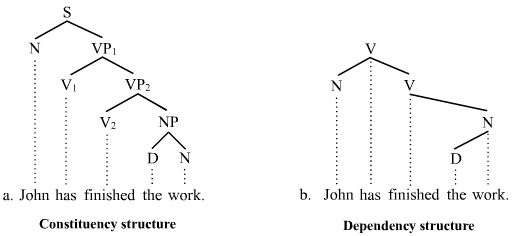
\includegraphics[width=0.7\textwidth]{figures/Johnhasfinishedthework}
	\caption{Parses of the sentence \textit{"John has finished the work"} \cite{parsers}}
	\label{fig:johnfinished}
\end{figure*}
%-------------------------------------------------------------
\section{Objectives}
The main focus of this study is computational semantics. My research includes building explicit representations of natural language semantics, because in today's state-of-the art systems for popular semantics tasks such as measuring semantic similarity or machine comprehension, they are rarely present. Virtually all systems
competing at popular challenges (e.g. \cite{Cer:2017,Collados:2017}) rely on word embeddings as the sole representation of word meaning. Recently \cite{Recski:2016c} has presented a method using graphical representations of natural language text that improved over the state-of-the art on the task of
measuring semantic similarity of pairs of English words. In this thesis
I use similar graphs as simple but powerful tools for measuring textual
entailment. My task includes defining new inference rules and methods for measuring graph similarities, and building an online available service for building graphs highly automatically, giving us a tool for building strong baseline methods. My work was based upon measuring our models through various semantic tasks such as Knowledge base population or the state-of-the art system on the 2018 Semeval Task \textit{Machine comprehension using commonsense knowledge}.

\section{Results}
We present a novel method for recognizing entailment using semantic
graphs and apply it to the tasks:
\begin{itemize}
    \item Knowledge base population task (KBP)
    \item 2017 RepEval task on Natural language inference (NLI)
    \item 2018 Semeval task on Machine
    Comprehension (MC).
\end{itemize}
First we present a highly automated process of building concept graphs from raw text building a microservice.
For the tasks I used the automatically built Concept graphs using the REST-API I defined based on the semantic parsing system \texttt{4lang} \cite{Recski:2016d}.
In the case of the KBP task I present a set of pilot experiments for augmenting a generic, open-domain 
knowledge base using a graph-based lexical ontology of English and simple
inference rules yielding millions of new facts with high
accuracy (over 90\% according to manual evaluation), the result was already presented in \cite{Kovacs:2018}.
For the NLI and MC task a strong baseline is presented using only concept graphs achieving accuracy scores of $67.5\%$ and $68.3\%$ respectively.
Followed by an enhancement of a state-of-the art system
\cite{Wang:2018}, where we proceeded to use the metric underlying our baseline as an additional feature. Preliminary results suggest that these features achieve a .5 percentage point improvement over the original system. This result was the output of the combined work with G\'emes Kinga presented in \cite{Kovacs:2018b}.

\section{References}
The code of the system is available on Github\footnote{\url{https://github.com/adaamko/4lang}}. The code was implemented by the author of this paper based upon the \textbf{4lang} system.

\section{Structure}
The structure of the paper is the following:
\begin{itemize}
	\item \textbf{Chapter \ref{chap:Introdu}} describes the short history and motivation of the NLP applications, it also gives a short summary about the objectives of the thesis, and the results.
	\item \textbf{Chapter \ref{chap:semanticparsing}} gives a short introduction into the field of semantic parsing, and semantic models in general. It briefly explains the semantic parsing system \textbf{4lang}, and my process of automating the building of concept graphs, and the newly defined inference methods
	\item \textbf{Chapter \ref{chap:comprehension}} describes the baseline approach to the Machine Comprehension task, which achieved an accuracy score of $68.3\%$.
	\item \textbf{Chapter \ref{chap:deep}} gives an introduction into deep learning, focusing on the NLP tasks.
	\item \textbf{Chapter \ref{chap:yuanfudao}} presents our experiments with the state-of-the art system \textbf{Yuanfudao}. Our preliminary results show a .5 percent improvement over the original system.
	\item \textbf{Chapter \ref{chap:future}} summarizes our contributions and describes our ongoing/future work. It briefly discusses our plans for the follow-up, that was beyond the scope of this work.
\end{itemize}

\section{Division of labour}
This project was a product of the combined work of Kov\'acs \'Ad\'am and G\'emes Kinga. Kov\'acs \'Ad\'am was responsible for building the service to automate the process of building concept graphs (online demo available at \url{http://4lang.hlt.bme.hu}), and was mostly working on the baseline methods and defining new inference rules and metrics for the given tasks. G\'emes Kinga's main work involved applying the baseline to the state-of-the-art system Yuanfudao \cite{Wang:2018}\footnote{\url{https://github.com/GKingA/commonsense-rc}} and experiments with IRTGs briefly described in Chapter \ref{chap:future}\footnote{\url{https://github.com/GKingA/irtg}}.
%----------------------------------------------------------------------------
\chapter{Semantic models and parsing}
\label{chap:semanticparsing}
%----------------------------------------------------------------------------

In this chapter I first introduce applications, that use semantic models as an essential knowledge for their process. After, the theory and problems of semantic representation are discussed, and I briefly present the upsides and downsides of such representations. After that we go into details about distributional and graph based models, introducing the semantic parsing system \textbf{4lang}, which is the main focus of our work. Finally, our micro-services are discussed, built around the parser to highly automate the process of building concept graphs from raw input. An easy example of their usage is shown as well.

When we use the word semantics, we usually refer to the interpretation of a linguistics unit (e.g. words, phrases, sentences, or whole texts) within the boundaries of a certain context. In many scientific fields e.g. philosophy, logic or biology the study of semantics is a highly researched task. While many NLP tasks like syntactic parsing, part-of-speech tagging, or even machine translation can be ignorant of the meaning of units, of what information they hold, there are also many other tasks that rely heavily on semantics.

Some examples, where semantic analysis is unavoidable:
\begin{itemize}
	\item \textbf{Question answering} is the process of generating meaningful answers to the user's question, using some kind of knowledge. It might be considered one of the oldest tasks in NLP or in AI in general with machine translation. With the recent rise of products like Siri, Alexa, or Watson, it is still one of the most researched area.
	\item \textbf{Recognizing entailment} is whether a statement implies another or not, it is closely connected to \textbf{machine comprehension}, which is the main focus of our work.
	\item \textbf{Chatbots} are systems, that somewhat can simulate the conversation of humans.
	\item \textbf{Sentiment analysis} is the task of understanding the opinion about a subject. Usually can be considered as a classification problem, where in the simplest case two class, "\textit{negative}" and "\textit{positive}" is given. More complex version of the task is also present, where the detection of the target of the opinion is also the part of the problem. There are solutions for the problem with hand-crafted rules and machine learning algorithms as well.  
\end{itemize}

For modeling the meaning of linguistic units, choosing an appropriate representation of our model is needed. While for syntactic analysis widely accepted concepts and ideas (e.g. dependency tree, phrase structure trees) of such representation are already in use, for a semantic model it still remained a challenging task. Even answering the question \textit{"What is a semantic representation?"} is not well defined, and mostly decided by the nature of our task. The units of a semantic model are also not globally decided (word, phrase or a sentence?).

Finding an absolute representation of semantics knowledge is among the most difficult task in Artificial Intelligence (AI). While we are yet to find a representation that has no downside, various experimental models are present, that are applicable for certain domains, but are problematic in other scenarios. So before choosing one, we need to take into account the limitations of each choice. 


Representation of semantic knowledge with logical expressions (e.g. zero-order logic, prepositional logic) exists, and although many companies still rely on hand-crafted rules as a knowledge representation, they are very unpractical and have serious problems with scalability and automation. Distributional models have risen in popularity in recent years, where meaning is represented with multi-dimensional vectors. While vector based models can give us a uniform representation, they mostly lack interpretability in a way that we never really know what happens inside these models. Another issue is the choice of the dimension. Many algorithms exist for reducing the dimension of such vectors to a fixed number, but determining the correct length can be difficult. Rare words are a big issue as well, if a word in the training data is rarely present, distributional models will fail to handle them correctly.

On the other hand, graph based solutions have high level of interpretability, and handling rare words is one of their biggest advantage. But automating the process of building graphs is a challenging task, and using them as a sole solution for a semantic parsing task in most cases would come short, but in hybrid systems they make up for the weaknesses other models have.

 In the next sections I will briefly discuss graph based models and distributional models, and because both of them have their merits, it is necessary to know the strengths and weaknesses of each one. My work focuses around graph based solutions.

\section{Distributional model}
In the field of natural language processing one way of encoding semantic meaning is to use distributional models. They model semantic meaning as real-valued vectors. These vectors need to be constructed from a training data, and we can calculate similarity as cosine distance between the vectors.

Let's have a look at these two sentences \textit{"The cat is walking in the bedroom"} and \textit{"A dog was running in a room"}. Words \textit{"dog"} and \textit{"cat"} have a similar semantic meaning, so if they are represented by vectors, and their cosine distance from each other is small, then we can vary the sentences \textit{"The dog is walking in the bedroom"} and \textit{"A cat was running in a room"} \cite{Bengio:2003}. These models take surrounding words into account and their goal is to obtain the meaning of the target word from their surroundings\cite{Jurafsky:2018}, and because \textit{"dog"} and \textit{"cat"} are close in vector space, they most likely will appear in the same context. This intuition helps us generalize sentences. These meanings are represented by vectors, called embeddings. One of the first models built around these intuitions were introduced in \cite{Bengio:2003}. 

These word embeddings are used in basically all state-of-the art systems related to natural language processing applications. Mikolov \cite{Mikolov:2013c} showed that word embeddings can be applied for vector operations, like addition or subtraction, and these operations often result in meaningful representation. If we have example words "\textit{King}", "\textit{Man}", "\textit{Woman}", then the vector("King") - vector("Man") + vector("Woman") \ref{fig:vecs} will most likely result in vector that is close to vector("Queen") in the embedding space.

 While the usage of word embeddings brought an important breakthrough in modeling word meaning, applying them for bigger linguistics units like phrases, sentences or even whole text remained a difficult challenge even for nowadays. One of the biggest reasons for this is the additive aspect of these models: if we model A B C expression with vector v(A) + v(B) + v(C), then we represent "John killed Bill" and "Bill killed John" sentences in the same way. 

\begin{figure*}[h!]
	\centering
	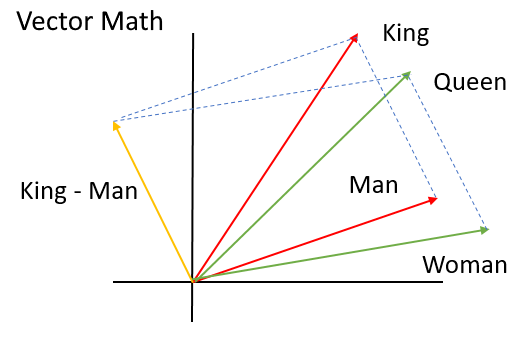
\includegraphics[width=0.7\textwidth]{figures/vecs}
	\caption{Vector addition example \cite{embeddings}}
	\label{fig:vecs}
\end{figure*}

The other issue is that we know very little about the structure of a multi-dimensional real-value vectors (for embeddings it can be from 300 up to 1000 dimension), so this makes it very hard to understand their structure, and exactly in what scenario they work, and the reason when they don't. So while most state-of-the art systems use word embeddings as a sole representation of meaning, and while it can be useful to encode meaning as vectors, so it can create connection from language specific and non-language specific data, we cannot deny the importance of having other semantics representations, such as graph-based ones. 

In the majority of my work, I researched graph-based solutions, where I model the meaning of linguistics unit with graphs, and the whole process can be defined with graph transformations. Next, I will briefly introduce graph based formalism starting with Abstract Meaning Representations (AMR) followed by the introduction of the \textbf{4lang} formalism, which will be the focus of the thesis, and I will go into details in the next section.

\section{Abstract Meaning Representations}
Abstract Meaning Representation (AMR) was introduced by Banarescu\cite{Banarescu:2013} for representing the meaning of linguistic structures. They represent meaning as directed acyclic graphs (DAGs), that can be used to capture the meaning of whole sentences. In the past few years, AMR related works have appeared e.g. parsing applications, or annotated corpuses \cite{Banarescu:2013, OGorman2018AMRBT, DAC:2017}.

Nodes of AMR graphs can be represented various ways. Each node in the graph represents a semantic concept \cite{AMR:2015}, that can be either an English word, or frameset from PropBank \cite{Palmer:2005}, essentially used for abstraction. The framesets are English verbs. The AMR introduced these variables for entities, events, properties, and states. An AMR can be converted to multiple formats:
\begin{itemize}
	\item Logic format
	\item AMR format
	\item Graph format
	
	These formats can be seen on Figure \ref{fig:amr} for sentence \textit{"the boy wants to go"}, and the corresponding 4lang representation on Figure \ref{fig:4langboy}.
	
\end{itemize}

\begin{figure*}[h!]
	\centering
	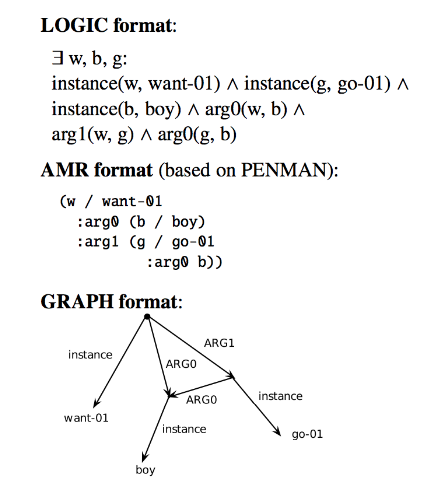
\includegraphics[height=0.4\textwidth]{figures/amr}
	\caption{Example sentence and representations \cite{Palmer:2005}}
	\label{fig:amr}
\end{figure*}

In this paper I use the semantic parser \textbf{4lang} \cite{Recski:2018}, and unlike \textbf{4lang}, AMR handles wider range of phenomenas, mostly typical of English. AMR's usage is mostly biased towards English \cite{Palmer:2005}, while 4lang can be configured to handle multiple languages.

\begin{figure*}[h!]
	\centering
	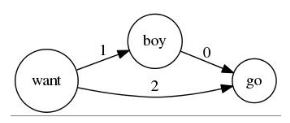
\includegraphics[width=0.3\textwidth]{figures/4langboy}
	\caption{Example sentence and representations in 4lang}
	\label{fig:4langboy}
\end{figure*}

In the next section, I will go into details about the \textbf{4lang} formalism, and the parser itself. After that I will describe our method of measuring similarities between semantic graphs, and its usage on semantic related tasks.

%----------------------------------------------------------------------------
\section{4lang}
\label{sec:4lang}
%---
The \textbf{4lang} system is in the main focus of my work, this section discussed the formalism and possible applications. \textbf{4lang} also means the manually built dictionary of mapping more than 2000 words to graphs, this is described in \cite{Kornai:2013}. After discussing the main formalism of \textbf{4lang}, I will demonstrate my highly automated process of building concept graphs, that was achieved by wrapping \textbf{4lang} functionality in micro-services building a REST-API, followed by our baseline for the machine comprehension task.

\subsection{The formalism}
The \texttt{4lang} system of semantic representation \cite{Kornai:2015a}
represents the meaning of linguistic units (both words and phrases)
as directed graphs of syntax-independent concepts. Every node of a \textbf{4lang} graph is a concept, which means that they are not taken as words, and they don't have any grammatical functions, like part-of-speech, voice, tense, etc.\cite{Recski:2016}.
Since these concepts have no grammatical attributes and no event structure, e.g.
the phrases \textit{water freezes} and \textit{frozen water} would both be
represented as \textit{water}~$\xrightarrow0$~\textit{freeze}. This also means that 4lang defines a many-to-one relation between the words and concepts. 

\textbf{4lang} formalism defines three types of edges:
\begin{itemize}
	\item \textbf{The 0-edge} represent represent attribution (\texttt{dog
		$\xrightarrow0$ large}), hypernymy (\texttt{dog $\xrightarrow0$ mammal}) and unary predication (\texttt{dog  $\xrightarrow0$ bark})
	\item \textbf{1- and 2-edges} those representing binary relations are connected to their arguments
	via edges labeled \texttt{1} and \texttt{2}, e.g \texttt{cat $\xleftarrow1$ catch $\xrightarrow2$ mouse}. Binaries that are shown with uppercase are binaries that must have two outgoing edges as shown in Figure \ref{fig:4langbin}. If we look at the sentence \textit{"Kinga broke Adam's bike"}, and the corresponding graph shown in Figure \ref{fig:4langbin}, if the 0-connection wouldn't be present between \textit{Kinga} $\xrightarrow0$ break, that would mean we consider that the relationship depend on whether the object of breaking is established or not. So in \textbf{4lang} the connection of 0-edge is present between a subject and a predicate regardless of the other arguments.
\end{itemize}

\begin{figure*}[h]
	\centering
	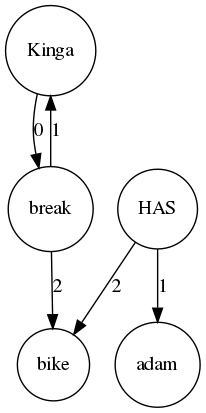
\includegraphics[height=0.5\textwidth]{figures/binary4lang}
	\caption{4lang with binaries}
	\label{fig:4langbin}
\end{figure*}

The example in
Figure~\ref{fig:bird} shows the \texttt{4lang} definition of the
concept \texttt{bird}. This definition was built manually, as part of
the \texttt{4lang} dictionary \cite{Kornai:2013}, but similar
definitions have been created automatically from definitions of
monolingual dictionaries such as Longman, using the
\texttt{dict\_to\_4lang} tool \cite{Recski:2016d}.

The open-source \textbf{4lang} pipeline\footnote{\url{https://github.com/kornai/4lang}}
contains tools for generating
directed graphs from raw text by mapping dependency edges in the output of the
Stanford parser \cite{deMarneffe:2006} to \texttt{4lang} subgraphs over
concepts corresponding to each word of the original sentence. The Stanford parser builds a dependency tree from the raw text that captures the syntactical relations between the linguistics units. \textbf{4lang} graph construction involves mapping from these relations to \textbf{4lang} semantics graphs, assigning the dependencies to \textbf{4lang} subgraphs. The mapping is presented in Table \ref{table:mapping}, and an example is shown for sentence \textit{"I like swimming"} in Figure \ref{fig:swimmingdep}, where we can see the dependency tree coming out of the Stanford parser, and the corresponding 4lang graph is present in Figure \ref{fig:swimming}, where the mapping from the dependency tree to \textbf{4lang} graph is done. 

\begin{table}
	\centering
	%\small
	\begin{tabular}{lc}
		\toprule
		Dependency & Edge \\
		\midrule
		amod & \multirow{7}{*}{\edge{$w_1$}{0}{$w_2$}} \\
		advmod & \\
		npadvmod & \\
		acomp & \\
		dep & \\
		num & \\
		prt & \\
		\midrule
		nsubj & \multirow{4}{*}{\twoedges{$w_1$}{1}{0}{$w_2$}} \\
		csubj & \\
		xsubj & \\
		agent & \\
		\midrule
		dobj & \multirow{6}{*}{\edge{$w_1$}{2}{$w_2$}} \\
		pobj & \\
		nsubjpass & \\
		csubjpass & \\
		pcomp & \\ 
		xcomp & \\
		\midrule
		appos & \twoedges{$w_1$}{0}{0}{$w_2$} \\
		\midrule
		poss & \multirow{2}{*}{$w_2\xleftarrow1$ \texttt{HAS} $\xrightarrow2w_1$} \\
		prep\_of & \\
		\midrule
		tmod & $w_1\xleftarrow1$ \texttt{AT} $\xrightarrow2w_2$ \\
		\midrule
		prep\_with & $w_1\xleftarrow1$ \texttt{INSTRUMENT} $\xrightarrow2w_2$ \\
		\midrule
		prep\_without & $w_1\xleftarrow1$ \texttt{LACK} $\xrightarrow2w_2$ \\
		\midrule
		prep\_P & $w_1\xleftarrow1$ \texttt{P} $\xrightarrow2w_2$ \\
		\bottomrule
	\end{tabular}
	\caption{Mapping from Stanford dependency relations to \textbf{4lang} subgraphs \cite[p. 12.]{Recski:2018}.}
	\label{table:mapping}
\end{table}

\begin{figure*}[h]
	\centering
	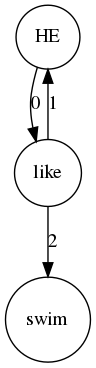
\includegraphics[height=0.5\textwidth]{figures/swimming}
	\caption{4lang example of a sentence}
	\label{fig:swimming}
\end{figure*}

\begin{figure*}[h]
	\centering
	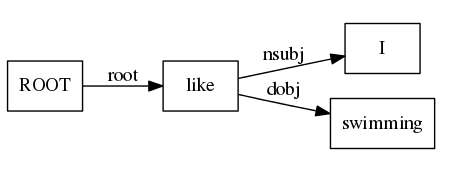
\includegraphics[width=0.5\textwidth]{figures/swimmingdep}
	\caption{Stanford example of a sentence}
	\label{fig:swimmingdep}
\end{figure*}


\subsection{Expansion}
Optionally, the \texttt{4lang} system allows us to \textit{expand}
graphs, a process which unifies the graph with the definition graphs of
each concept. The implementation is written in the \textbf{dict\_to\_4lang} module, that extends the functionality of the discussed \textbf{text\_to\_4lang} pipeline with dictionaries. \textbf{4lang} takes advantage of this, and implements the expansion step, which is essentially joining the definitions graphs to the main graph. This allows us to build a larger graph, that contains more information, and allows us to model the text better by simply adding the definition of words.

Let us look at the example sentence \textit{"My poor wife"}, that results the graph shown in Figure \ref{fig:mypoor}. Looking at the definition of the word \textit{poor}: \textit{having very little money and not many possessions}, we can build a definition graph and essentially join the two graphs together. This can result us a better model if we are ready to take word definitions into account, and with this method we can have higher similarities between graphs whose sentences are also similar \footnote{Of course not every interpretation of \textit{"poor"} is related to money. It requires a higher level mechanism to handle these kind of occurrences, see more in \cite{Kornai:2018}.}. Doing this for every word in the sentence resulting in a merged graph Figure \ref{fig:mypoorexpanded}. If we look at the graph, it is clear that the expanded graph gives us much more accurate context and definition. My work was built around the expanded graph, and enhancing it with inference rules. We will see that how better it actually performs on a real task. This will be the main topic of Chapter \ref{nli}.

\begin{figure}
	\centering
	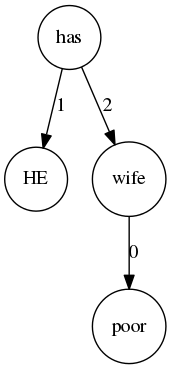
\includegraphics[scale=0.5]{figures/mypoor}
	\caption{4lang definition of sentence \textit{"My poor wife"}.}
	\label{fig:mypoor}
\end{figure}

\begin{figure}
	\centering
	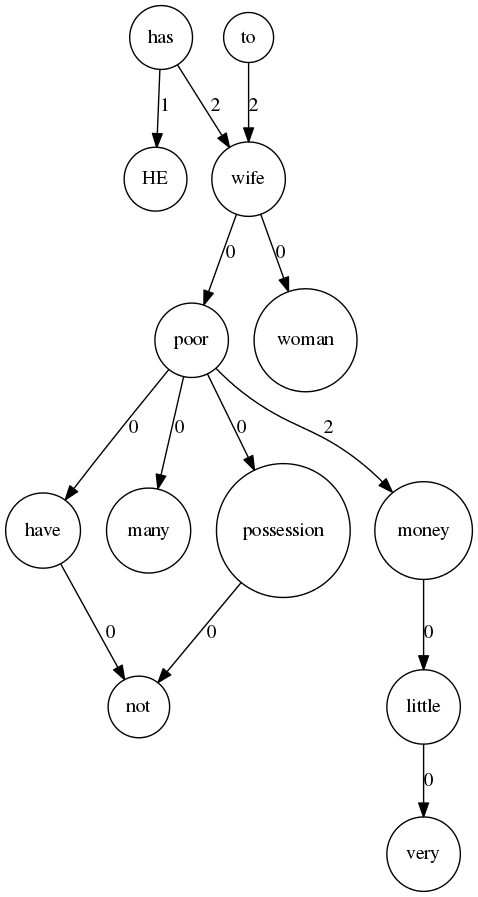
\includegraphics[scale=0.5]{figures/mypoorexpanded}
	\caption{4lang definition of expanded sentence \textit{"My poor wife"}.}
	\label{fig:mypoorexpanded}
\end{figure}


\subsection{The service}
At the beginning of my research I put a high emphasis on generating graphs from raw text with a highly automated method, so besides being an open-source software library, one of my contribution consists of the accessibility of \texttt{4lang} via a public
REST API at \url{http://hlt.bme.hu/4lang}. I used the python language for implementing the service, and for the framework I used the flask\footnote{http://flask.pocoo.org/} package. The service generates input for the \texttt{text\_to\_4lang} module from the raw text input, then after processing it, returns a graph in \textbf{networkx multigraph}\footnote{\url{https://networkx.github.io/documentation/networkx-1.9.1/reference/classes.multigraph.html}} format to make it easy to visualize it on essentially any client side. Online demo of the service is available at \url{http://4lang.hlt.bme.hu}. 
The process is presented in Example \ref{lst:code}.
\begin{center}
	\begin{lstlisting}[caption={Demonstration of the service in python language.},language=python, label={lst:code}]
sentence = "I like micro-services." 
data = {'sentence':   sentence}
data_json = json.dumps(data)
payload = {'json_payload': data_json}
headers = {'Content-type': 'application/json', 'Accept': 'text/plain'}
r = requests.post("http://hlt.bme.hu/4lang/sendef", 
data=data_json, headers=headers)
s_machines = r.json()['sentence']
\end{lstlisting}
\end{center}


The generated graph can be seen in Figure \ref{fig:service}. The code of the service is publicly available on Github\footnote{\url{https://github.com/adaamko/4lang}}. We can generate graphs with raw text by calling the service. Currently my service has multiple endpoints, with each of them representing different methods.
If you are only interested in processing a single sentence, the following endpoints are available:

\begin{figure}[!htb]
	\centering
	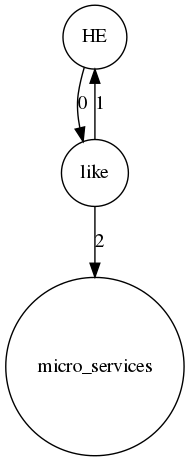
\includegraphics[scale=0.4]{figures/service}
	\caption{4lang definition of sentence \textit{"I like micro-services"}.}
	\label{fig:service}
\end{figure}

\begin{itemize}
	\item \textbf{/sendef} - Returns the graphs built from the sentence.
	\item \textbf{/senexp} - Returns the graphs, where the word's definition has been added to the graph.
	\item \textbf{/senabs} - Calling this function, with the help of simple inference rules, we can build more abstract graph that in certain scenarios can capture meaning in a different way than the expand function does. While the functionality is already implemented, it is yet to reach the results of the expansion method, so it can be described as a more of a future work, we will explain the method in Chapter \ref{chap:nli}.
\end{itemize}
You can get a word's definition by calling the defined endpoint:
\begin{itemize}
	\item \textbf{/definition} - Returns the graphs built from the word's definition.
\end{itemize}
For the machine comprehension task we defined a dedicated endpoint:
\begin{itemize}
	\item \textbf{/rally} - Returns a merged graph, where we merge a question sentence with an answer sentence. The main goal of this endpoint is that we can get a graph that can be explicitly compared with graph built from the passage text (it will be explained in Chapter \ref{chap:comprehension } concretely). 
\end{itemize}


\begin{figure}[!htb]
	\centering
	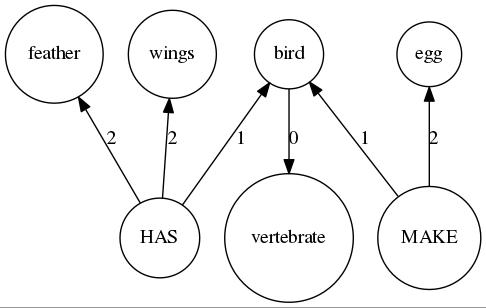
\includegraphics[scale=0.5]{figures/bird}
	\caption{4lang definition of \texttt{bird}.}
	\label{fig:bird}
\end{figure}

Graphs generated by the \texttt{4lang} parser have previously been used
successfully in measuring semantic similarity. The current state of the
art system on the \texttt{SimLex-999} benchmark \cite{Hill:2014a}
outperforms previous top systems by utilizing a simple similarity metric
between \texttt{4lang} definitions of pairs of English words
\cite{Recski:2016c}, this was the main idea of trying it in a different task with a different state-of-the-art system.

In the next chapter, I will briefly discuss the main challenges we chose for evaluation, mainly the task of KBP. After, I will introduce our baselines methods for solving the NLI and MC tasks using our micro-service for automatically building concept graphs. Finally I will present our mutual work, where we made it applicable to an already working system.
%----------------------------------------------------------------------------
\chapter*{Acknowledgement}\addcontentsline{toc}{chapter}{Acknowledgement}
%----------------------------------------------------------------------------
First of all, 
I would like to express my deep gratitude to Dr. Recski G�bor for his guidance not just through this thesis, but through my whole master studies. I would like to thank him for introducing me to this interesting and amazing research field. He was always flexible and available for all my questions. I thank him for his valuable advices just about any topic imaginable.  

I am also thankful to Dr. Kornai Andr�s for his constant support
and help with my work. I thank him for his energy to discuss any of problems I have.

I also would like to thank to my colleague G�mes Kinga for her excellent work. 

Finally, a special thanks to my girlfriend for her constant love and support. I thank her for her supporting me even through difficult situations. Without her, I would not have been able to write this thesis.

%\listoffigures\addcontentsline{toc}{chapter}{?br?k jegyz?ke}
%\listoftables\addcontentsline{toc}{chapter}{T?bl?zatok jegyz?ke}

\bibliography{mybib}
\addcontentsline{toc}{chapter}{Bibliography}
\bibliographystyle{plain}

\label{page:last}
\end{document}
